% Chapter Template


\chapter{Chapter Title Here} % Main chapter title
%\chapter[toc version]{doc version}
%\chaptermark{version for header} %Short version of the title for the headeer
\label{ChapterX} % Change X to a consecutive number; for referencing this chapter elsewhere, use \ref{ChapterX}

% Write text in here
% Use \subsection and \subsubsection to organize text

Welcome to the tutorial on how to use this thesis model. This is not to teach you how to use \LaTeX. For that read a tutorial. But this aims to teach you how to do the basic stuff you will need in order to produce a decent document.

\section{Citations}
You can add extra info to you references, like \cite[chapter 3]{Nobody06}

\section{Figures}

Let us start with a figure with two subfigures like in \ref{fig:FCUPfatCat}. 

\begin{figure}
	\centering
	\begin{subfigure}{.49\textwidth}
  		\centering
  		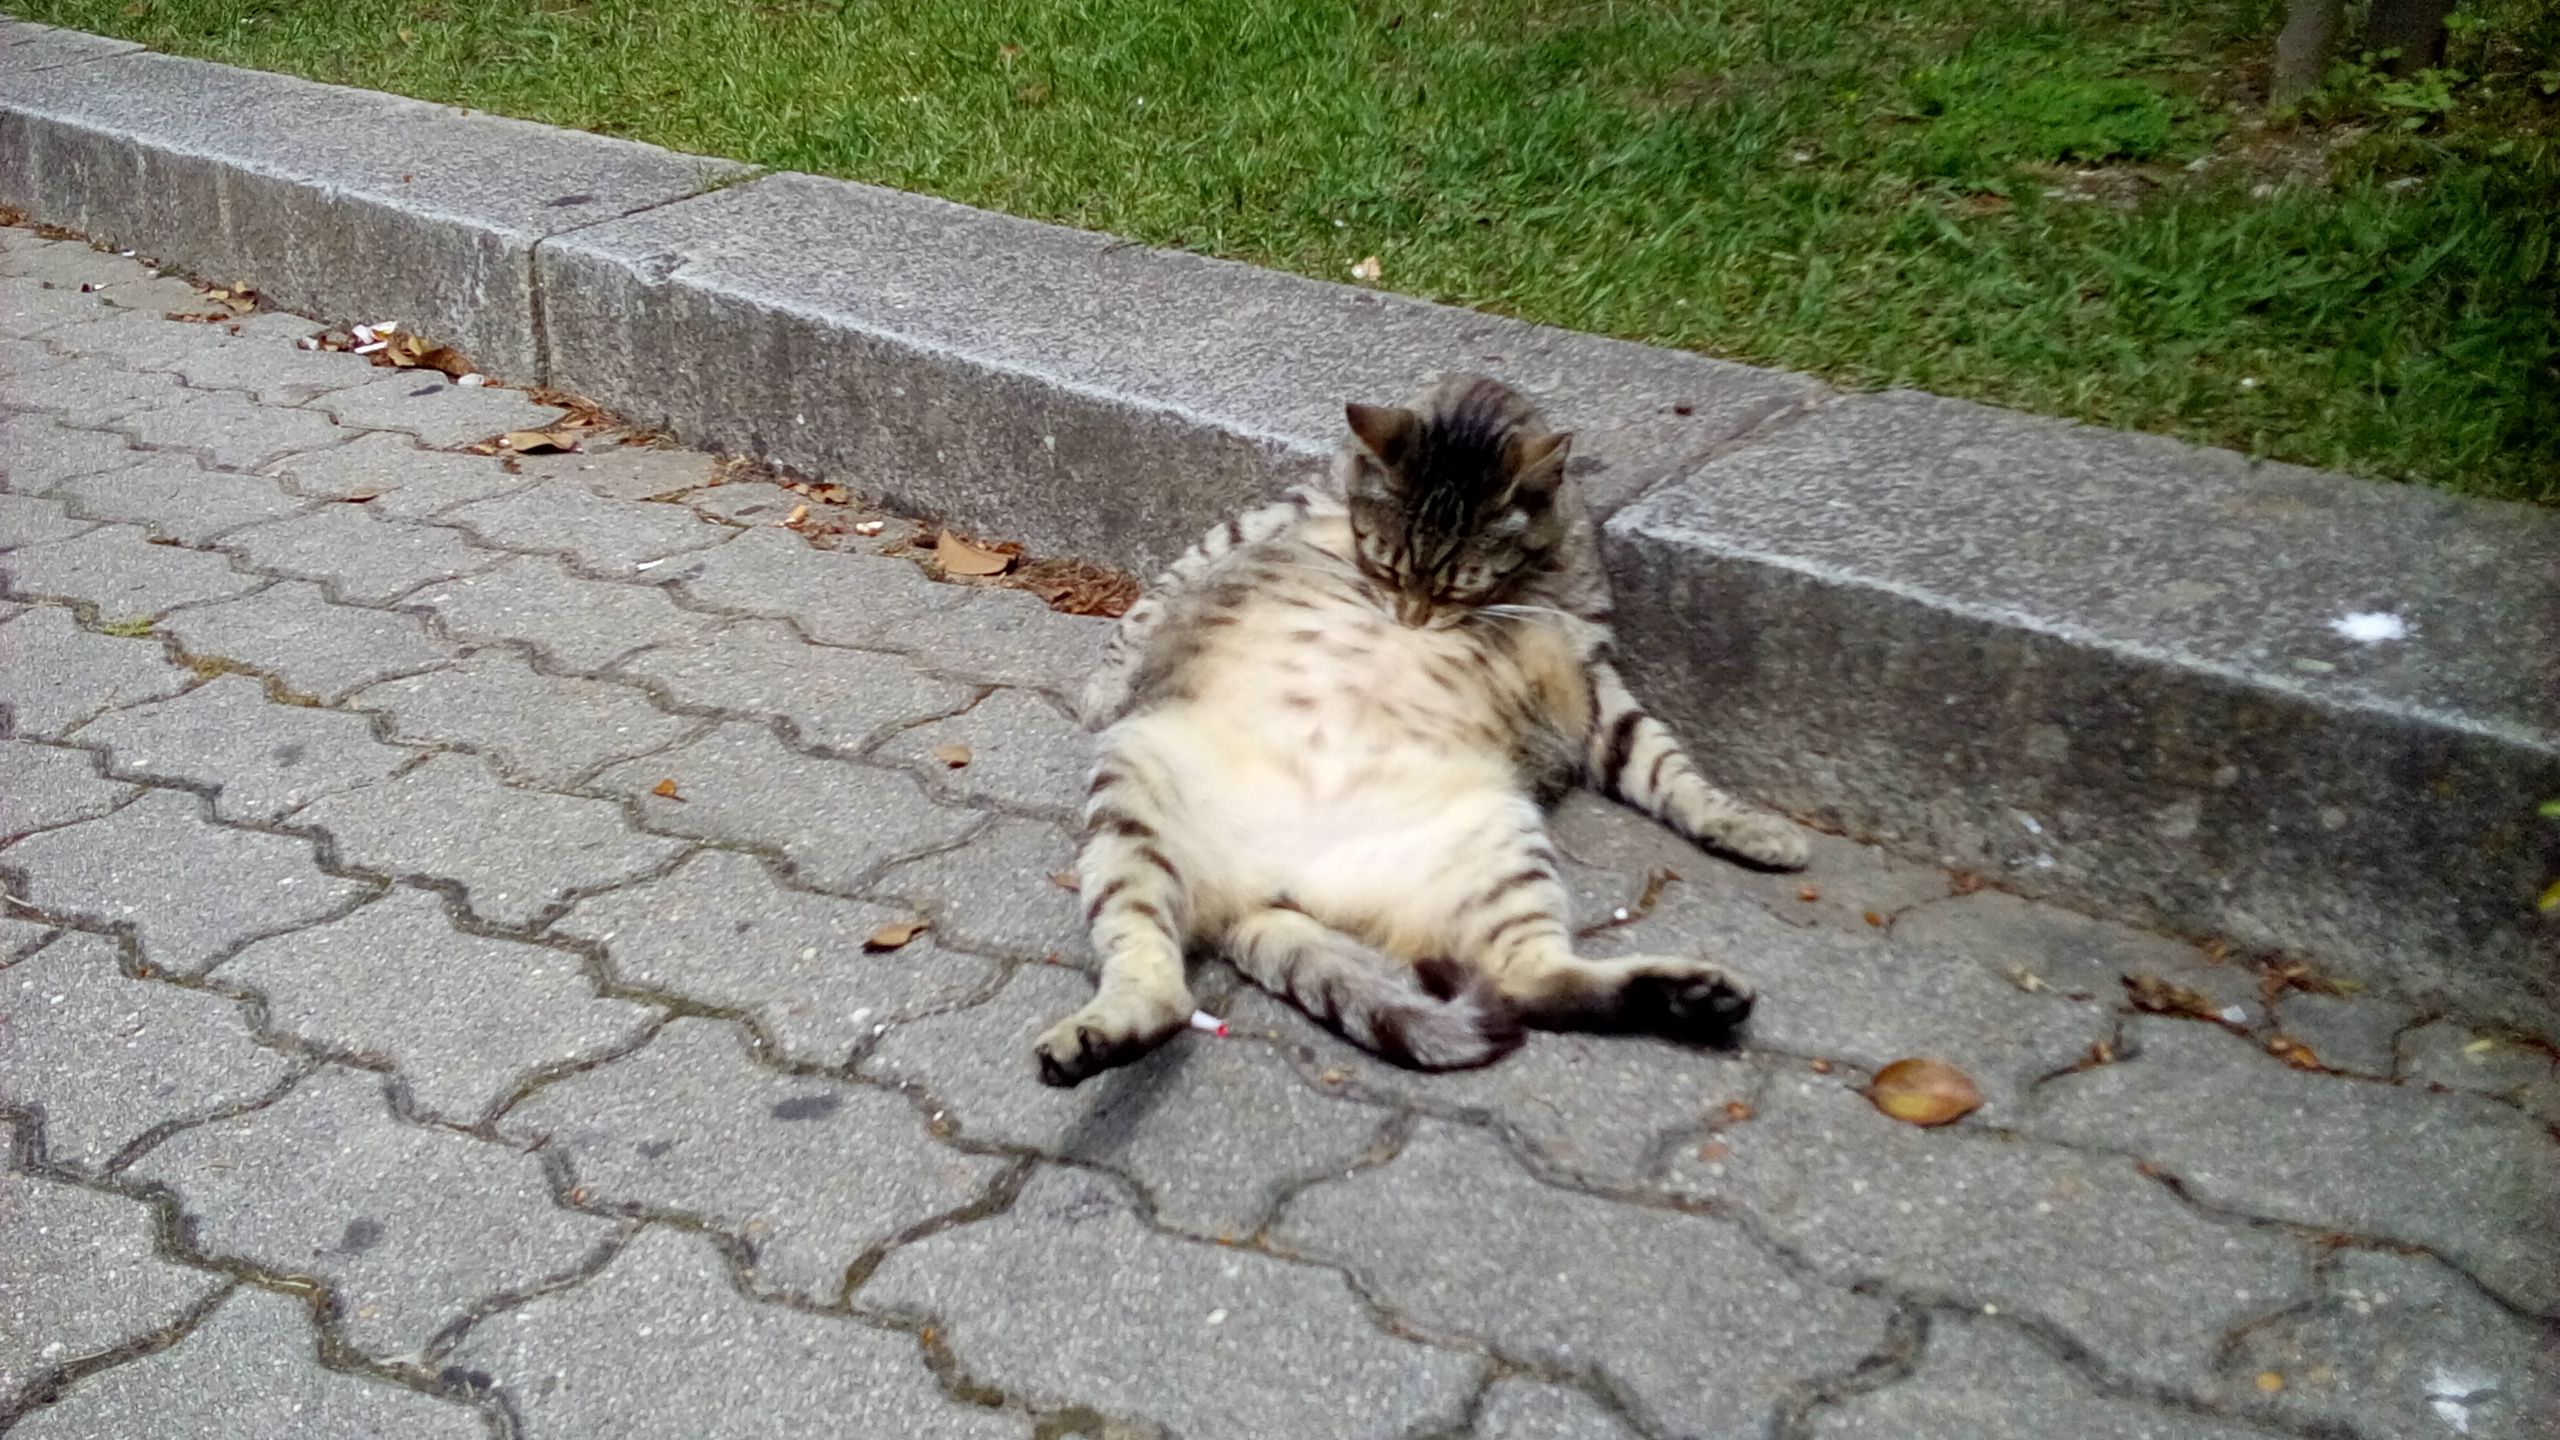
\includegraphics[width=.95\linewidth]{Figures/ChapterTemplate/20160517_123603.jpg}
  		\caption{FCUP's fat cat doing what cats do.}
	\end{subfigure}%
	\hfill
	\begin{subfigure}{.49\textwidth}
  		\centering
 		 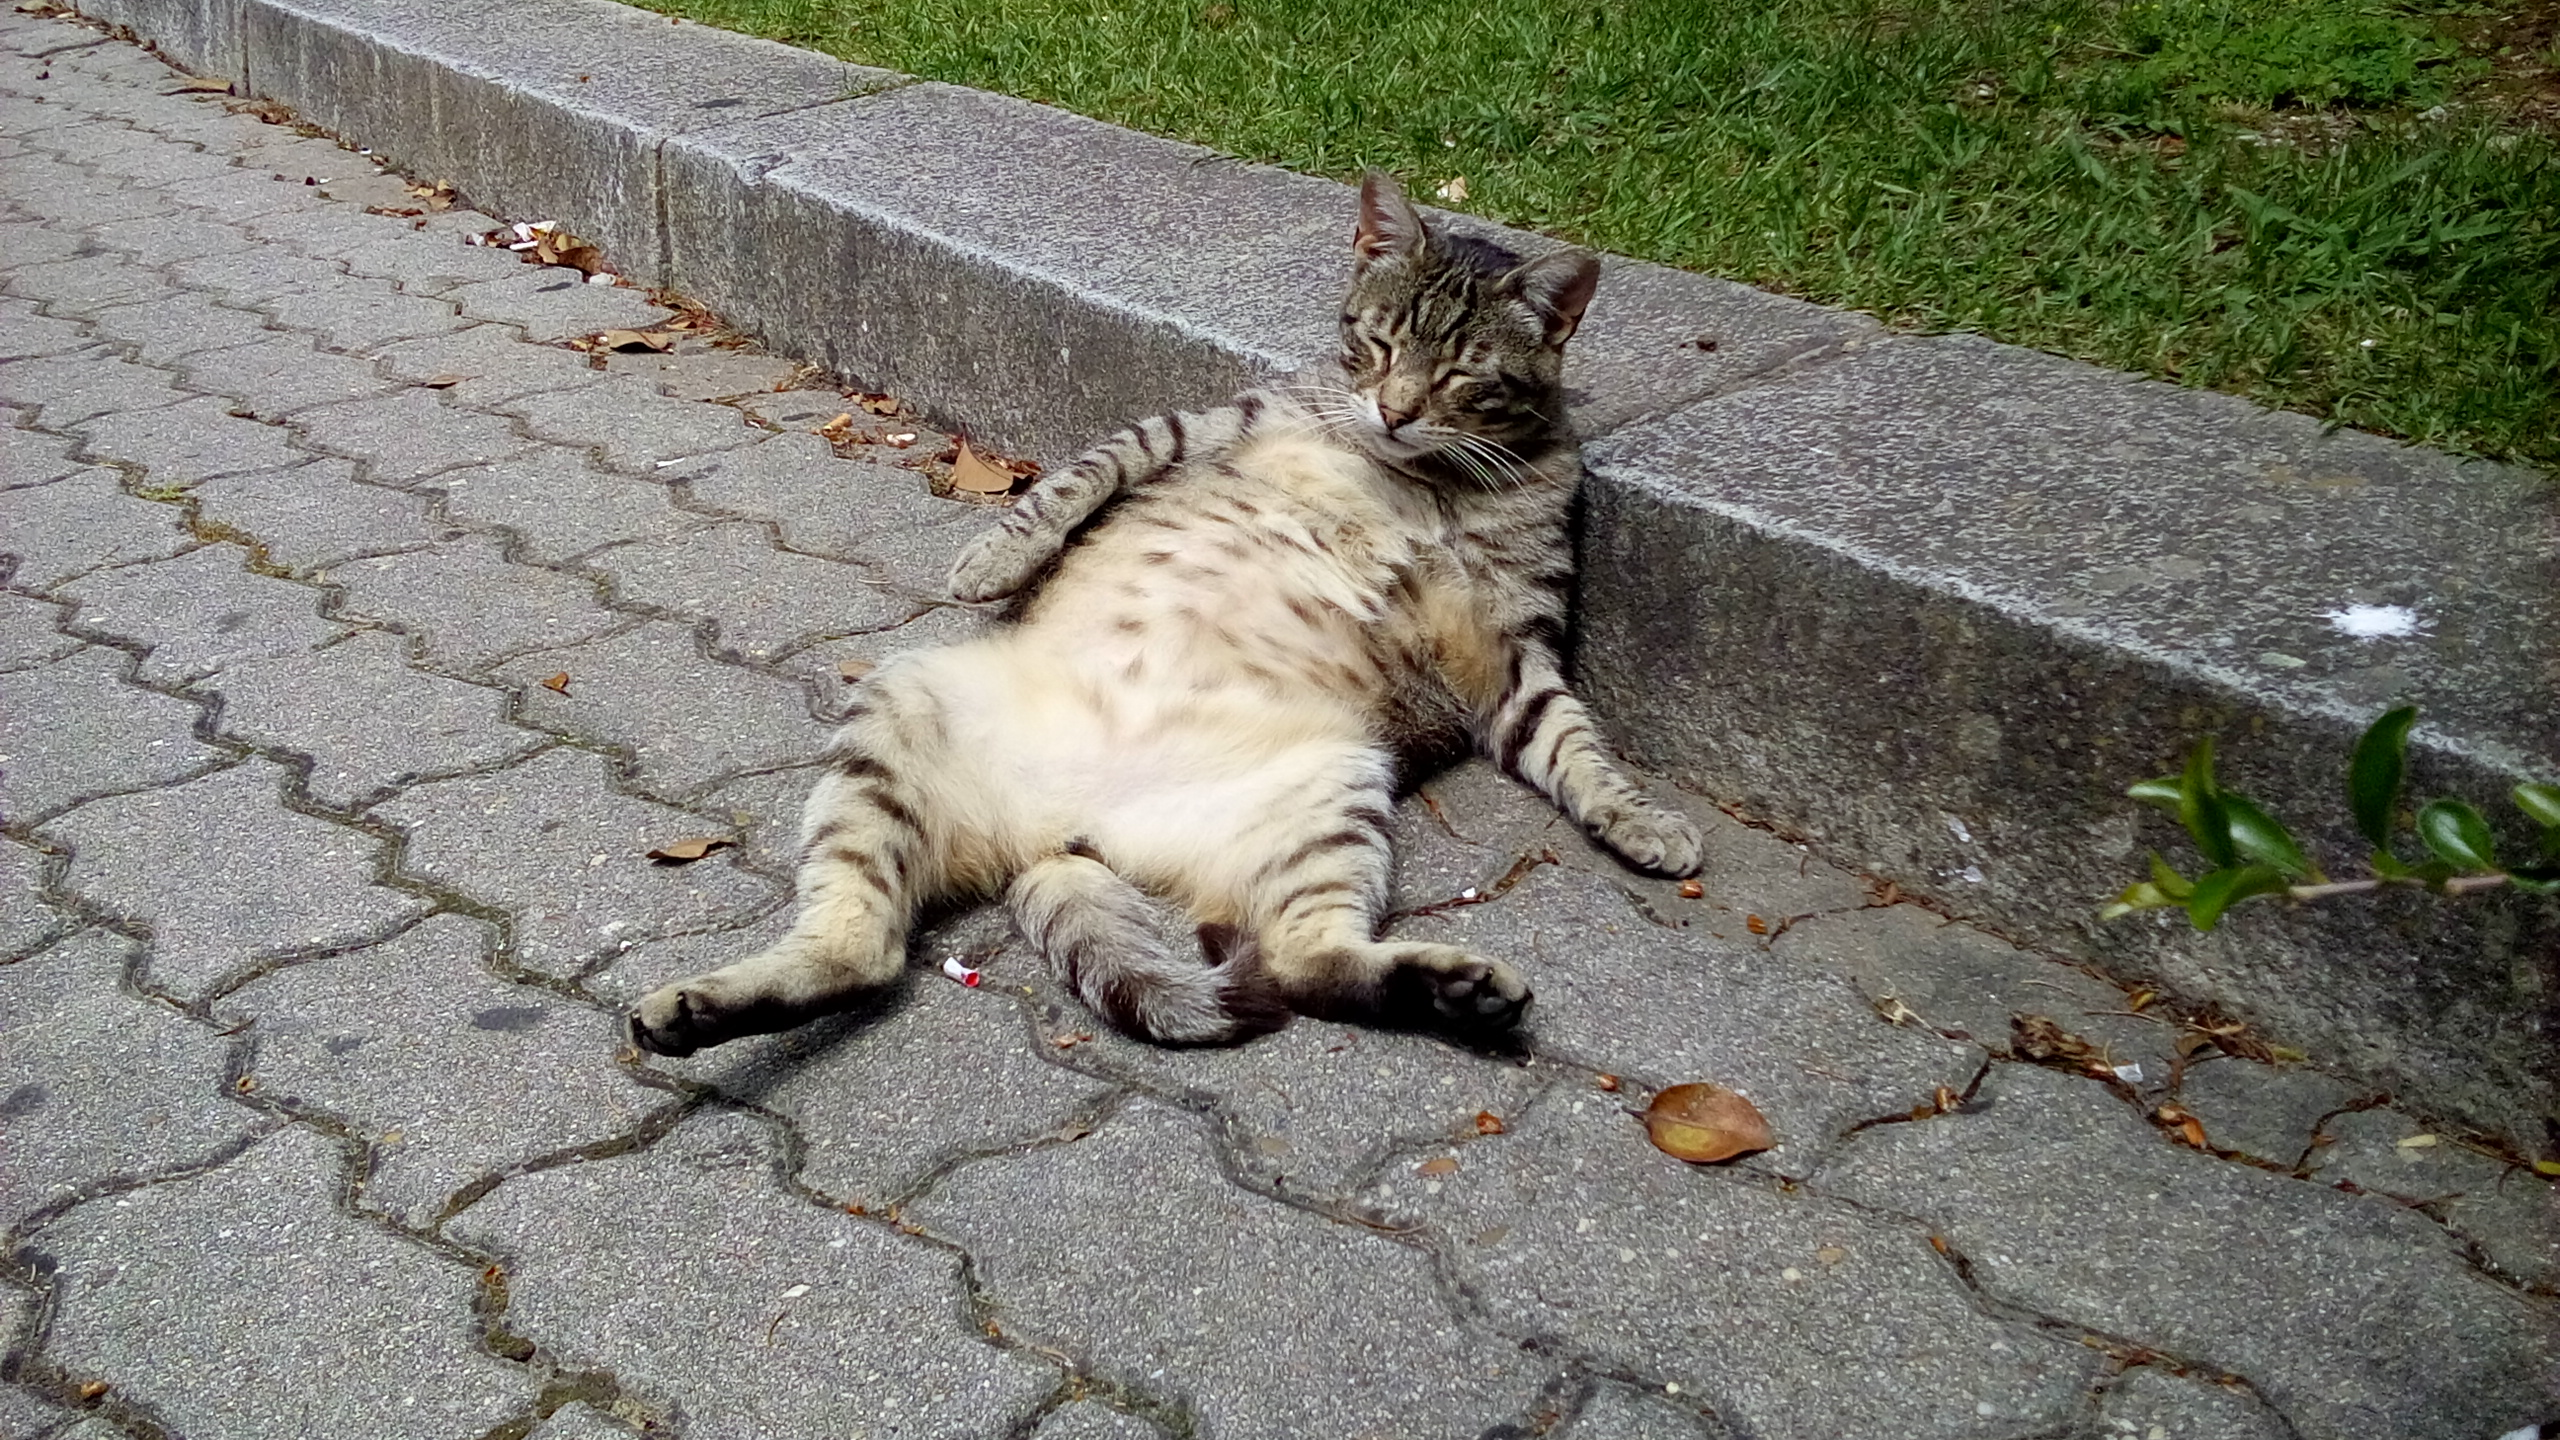
\includegraphics[width=.95\linewidth]{Figures/ChapterTemplate/20160517_123609.jpg}
 		 \caption{FCUP's fat cat resting.}
	\end{subfigure}
	\caption{\label{fig:FCUPfatCat}FCUP's fat cat.} 
\end{figure}


Or two figures side by side like \ref{fig:FCUPfatcatSide1} and \ref{fig:FCUPfatcatSide2}.

\begin{figure}
\centering
\begin{minipage}{.49\textwidth}
  \centering
  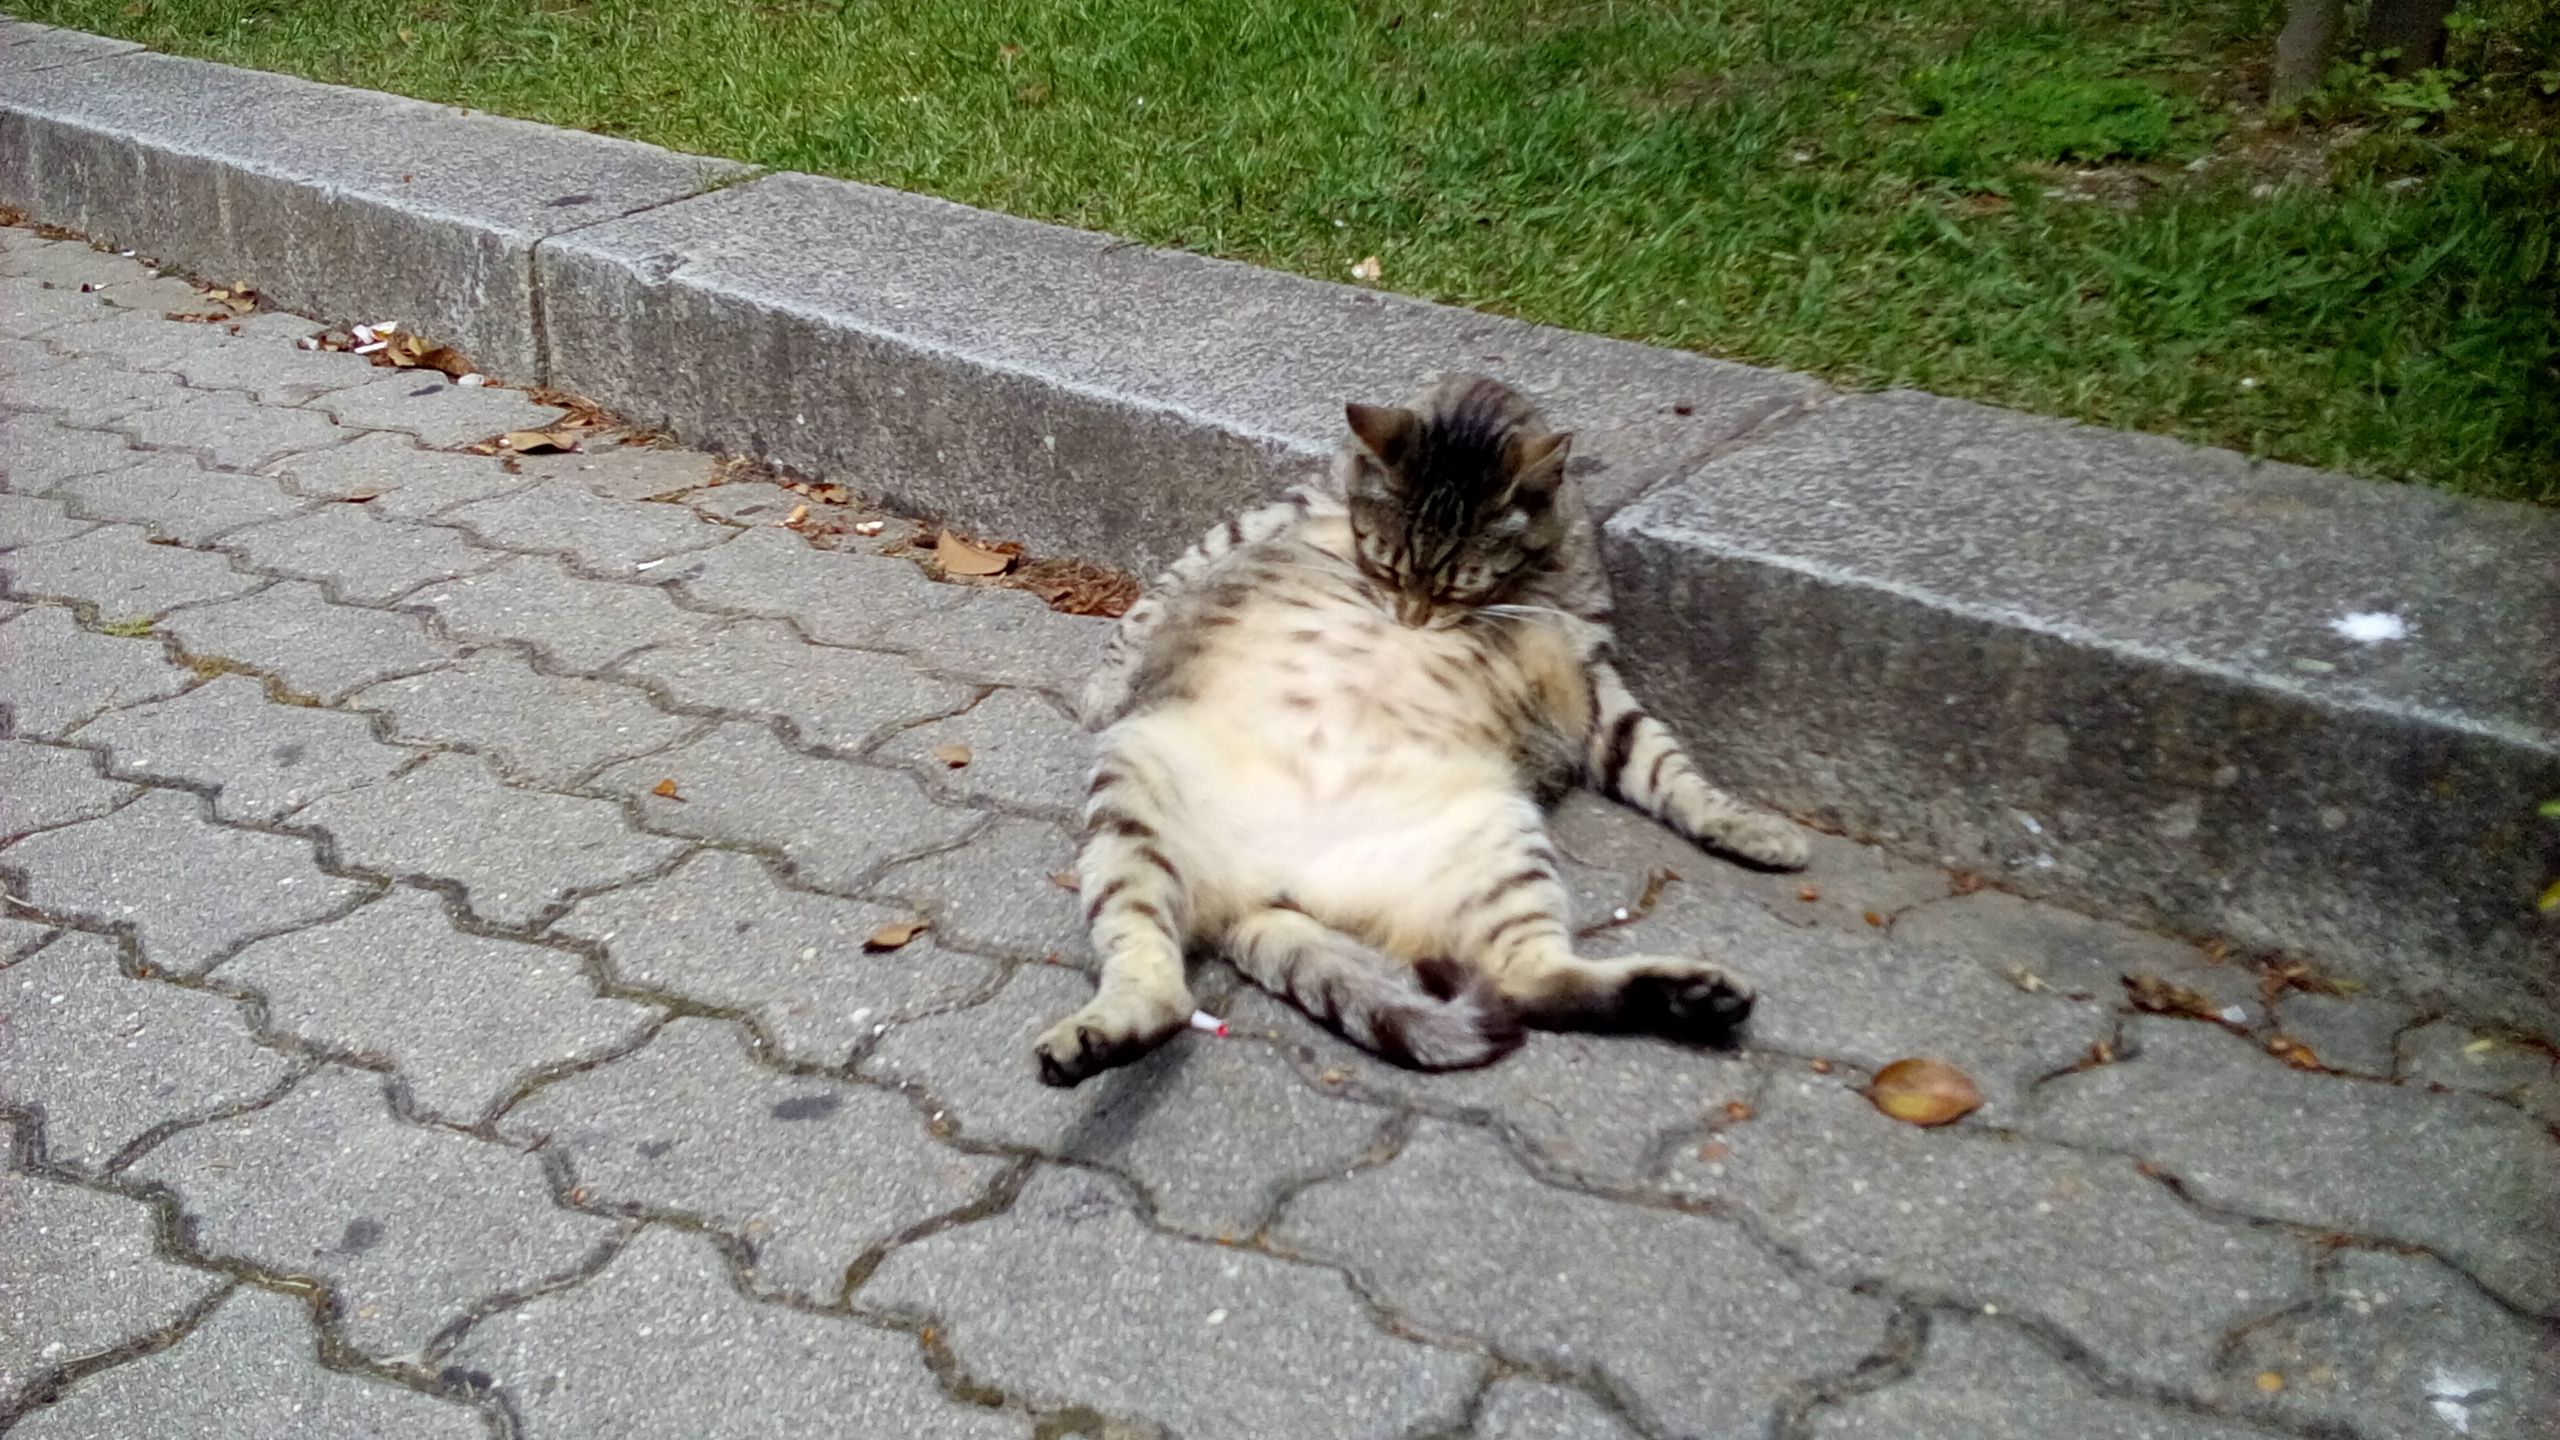
\includegraphics[width=.95\linewidth]{Figures/ChapterTemplate/20160517_123603.jpg}
  \captionof{figure}{\label{fig:FCUPfatcatSide1}FCUP's fat cat doing what cats do.}
\end{minipage}%
\hfill
\begin{minipage}{.49\textwidth}
  \centering
  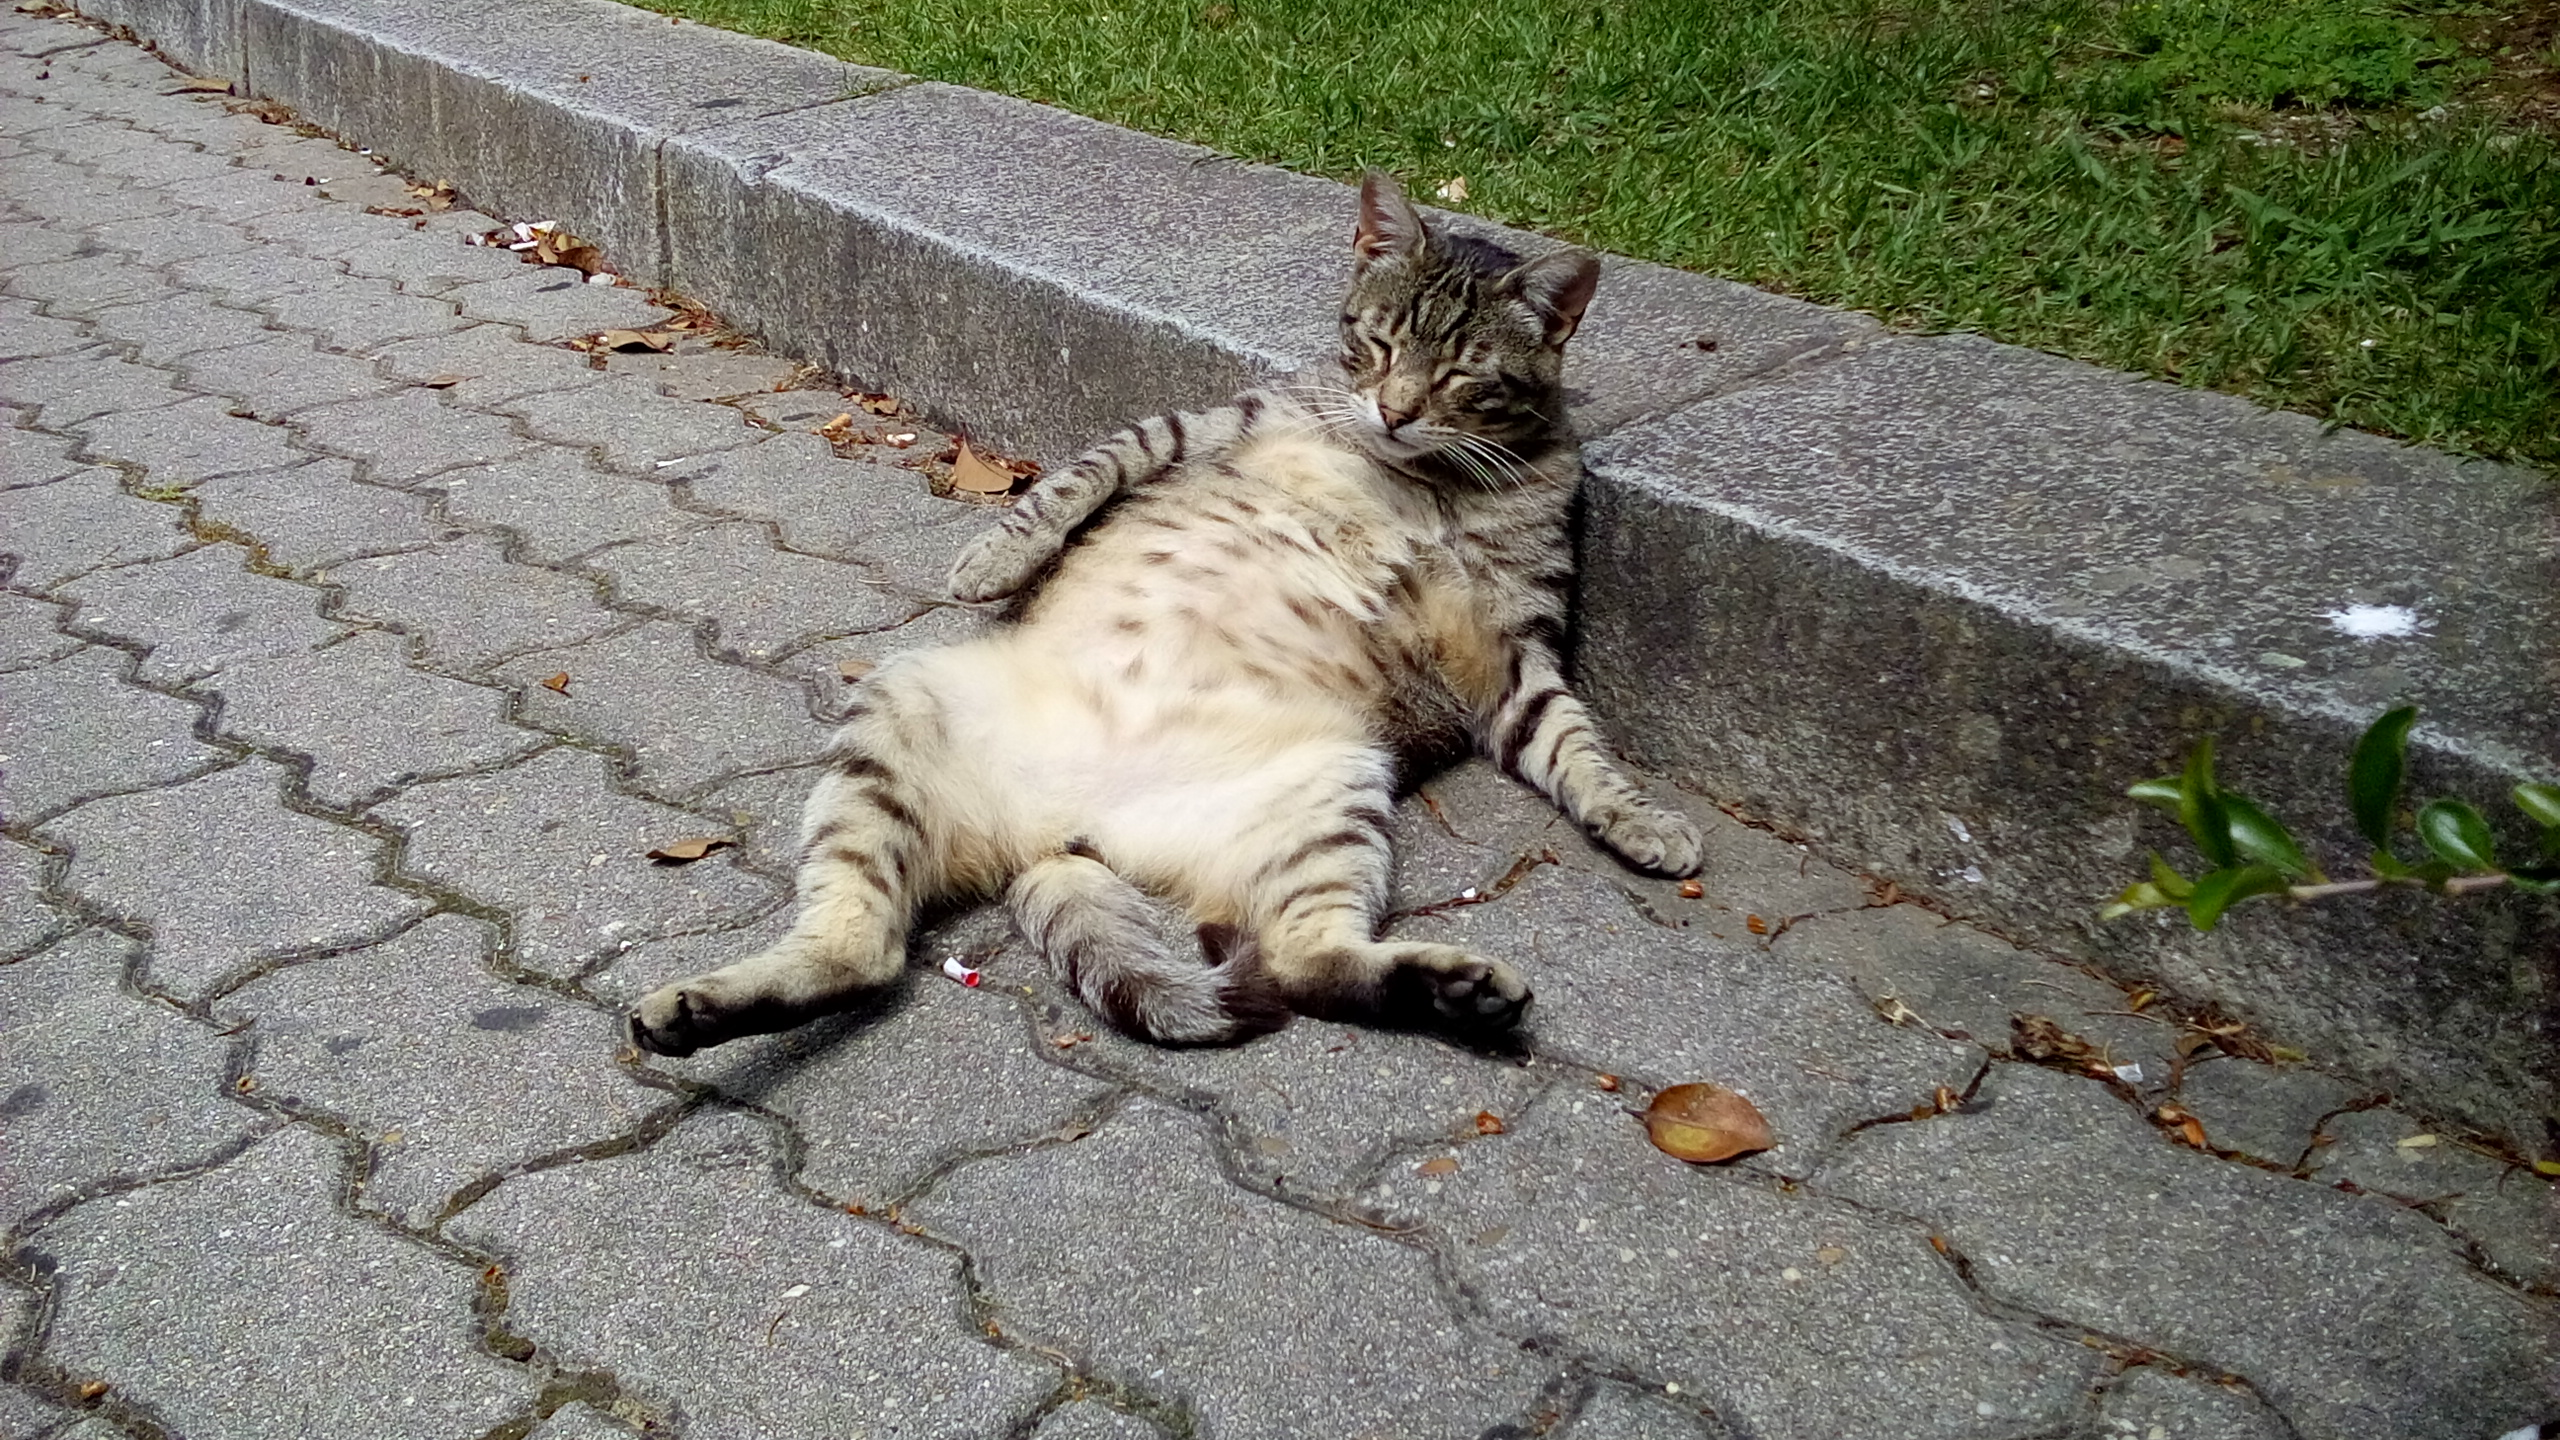
\includegraphics[width=.95\linewidth]{Figures/ChapterTemplate/20160517_123609.jpg}
  \captionof{figure}{\label{fig:FCUPfatcatSide2}FCUP's fat cat.} 
\end{minipage}
\end{figure}


Or a figure with some text on the side, like \ref{fig:FCUPfatcatSide3}, or even a Figure wrapped around in text, as seen on Figure \ref{fig:FCUPfatcatSide4}

\begin{figure}
\centering
\begin{minipage}{.49\textwidth}
  And here we have some text related to this image. The text can occupy the same space as the image would normally do...
\end{minipage}%
\hfill
\begin{minipage}{.49\textwidth}
  \centering
  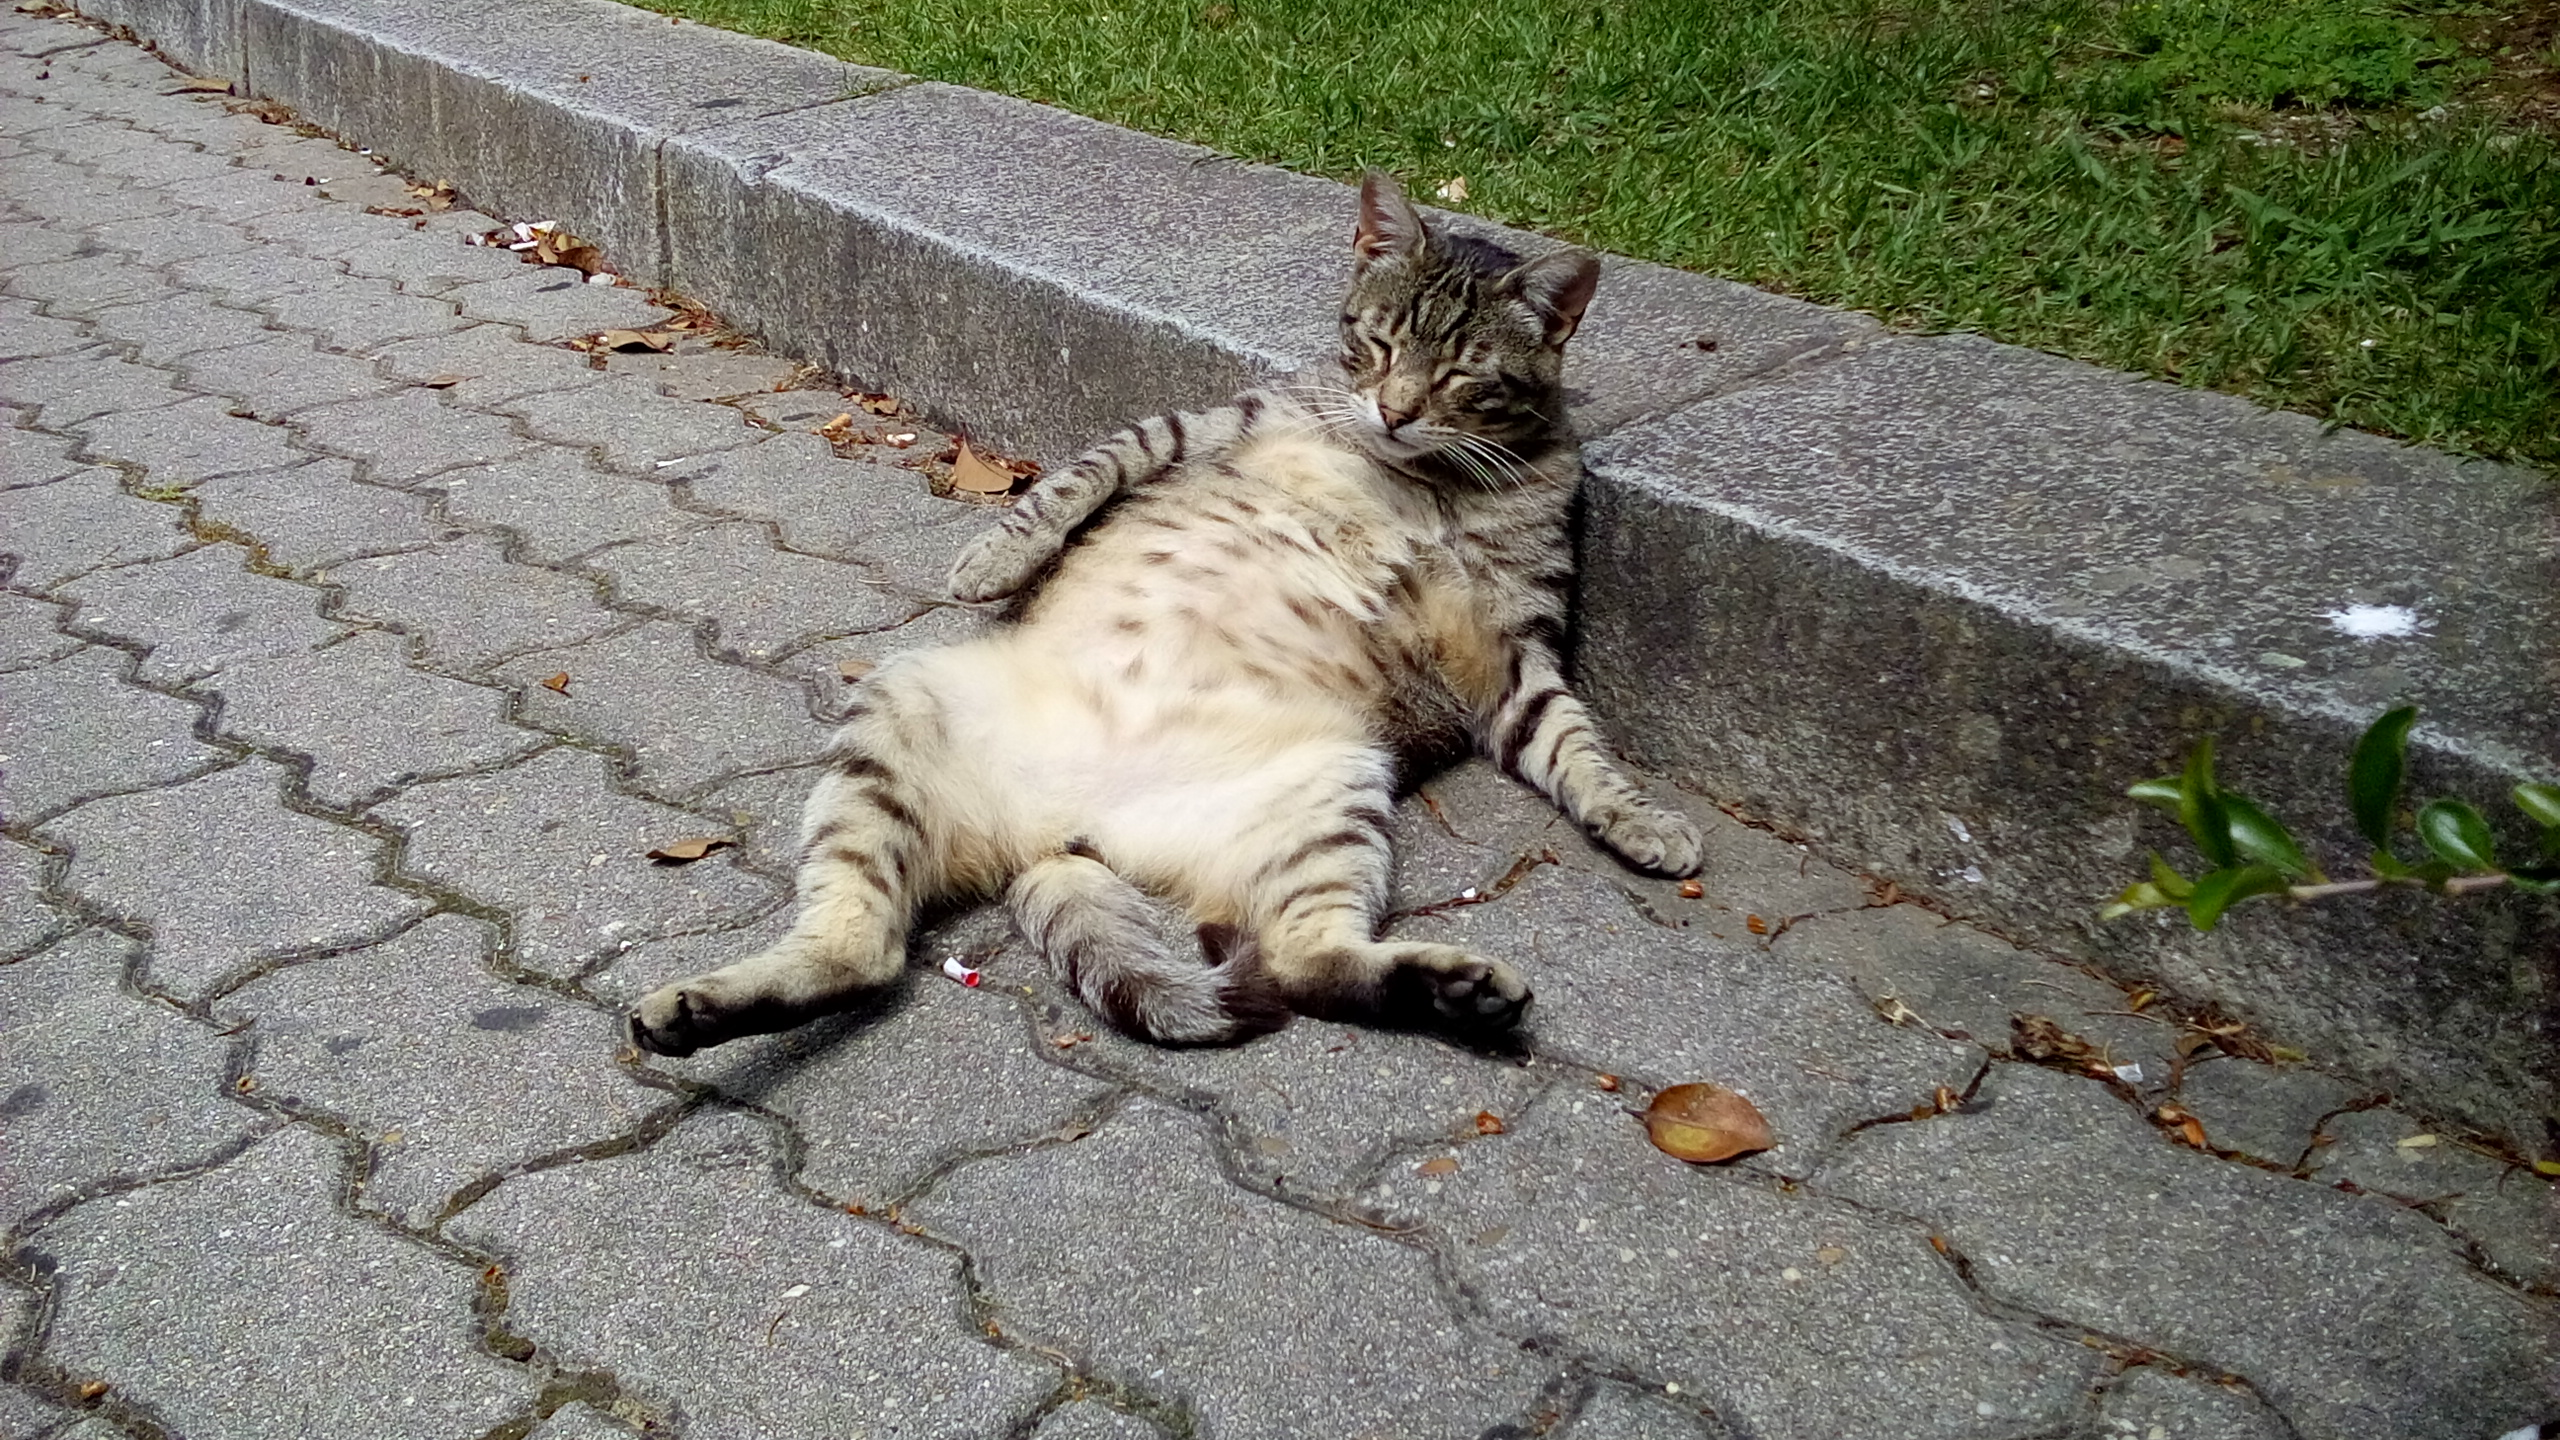
\includegraphics[width=.95\linewidth]{Figures/ChapterTemplate/20160517_123609.jpg}
  \captionof{figure}{\label{fig:FCUPfatcatSide3}FCUP's fat cat.} 
\end{minipage}
\end{figure}

% If you find figures split between two pages, use the uppercase L or R, to let the wrapped figure be a float object that can move   through the page
This is where the table goes with text wrapping around it. You may 
embed tabular environment inside wraptable environment and customize as you like: 
\begin{wrapfigure}{r}{8cm}
  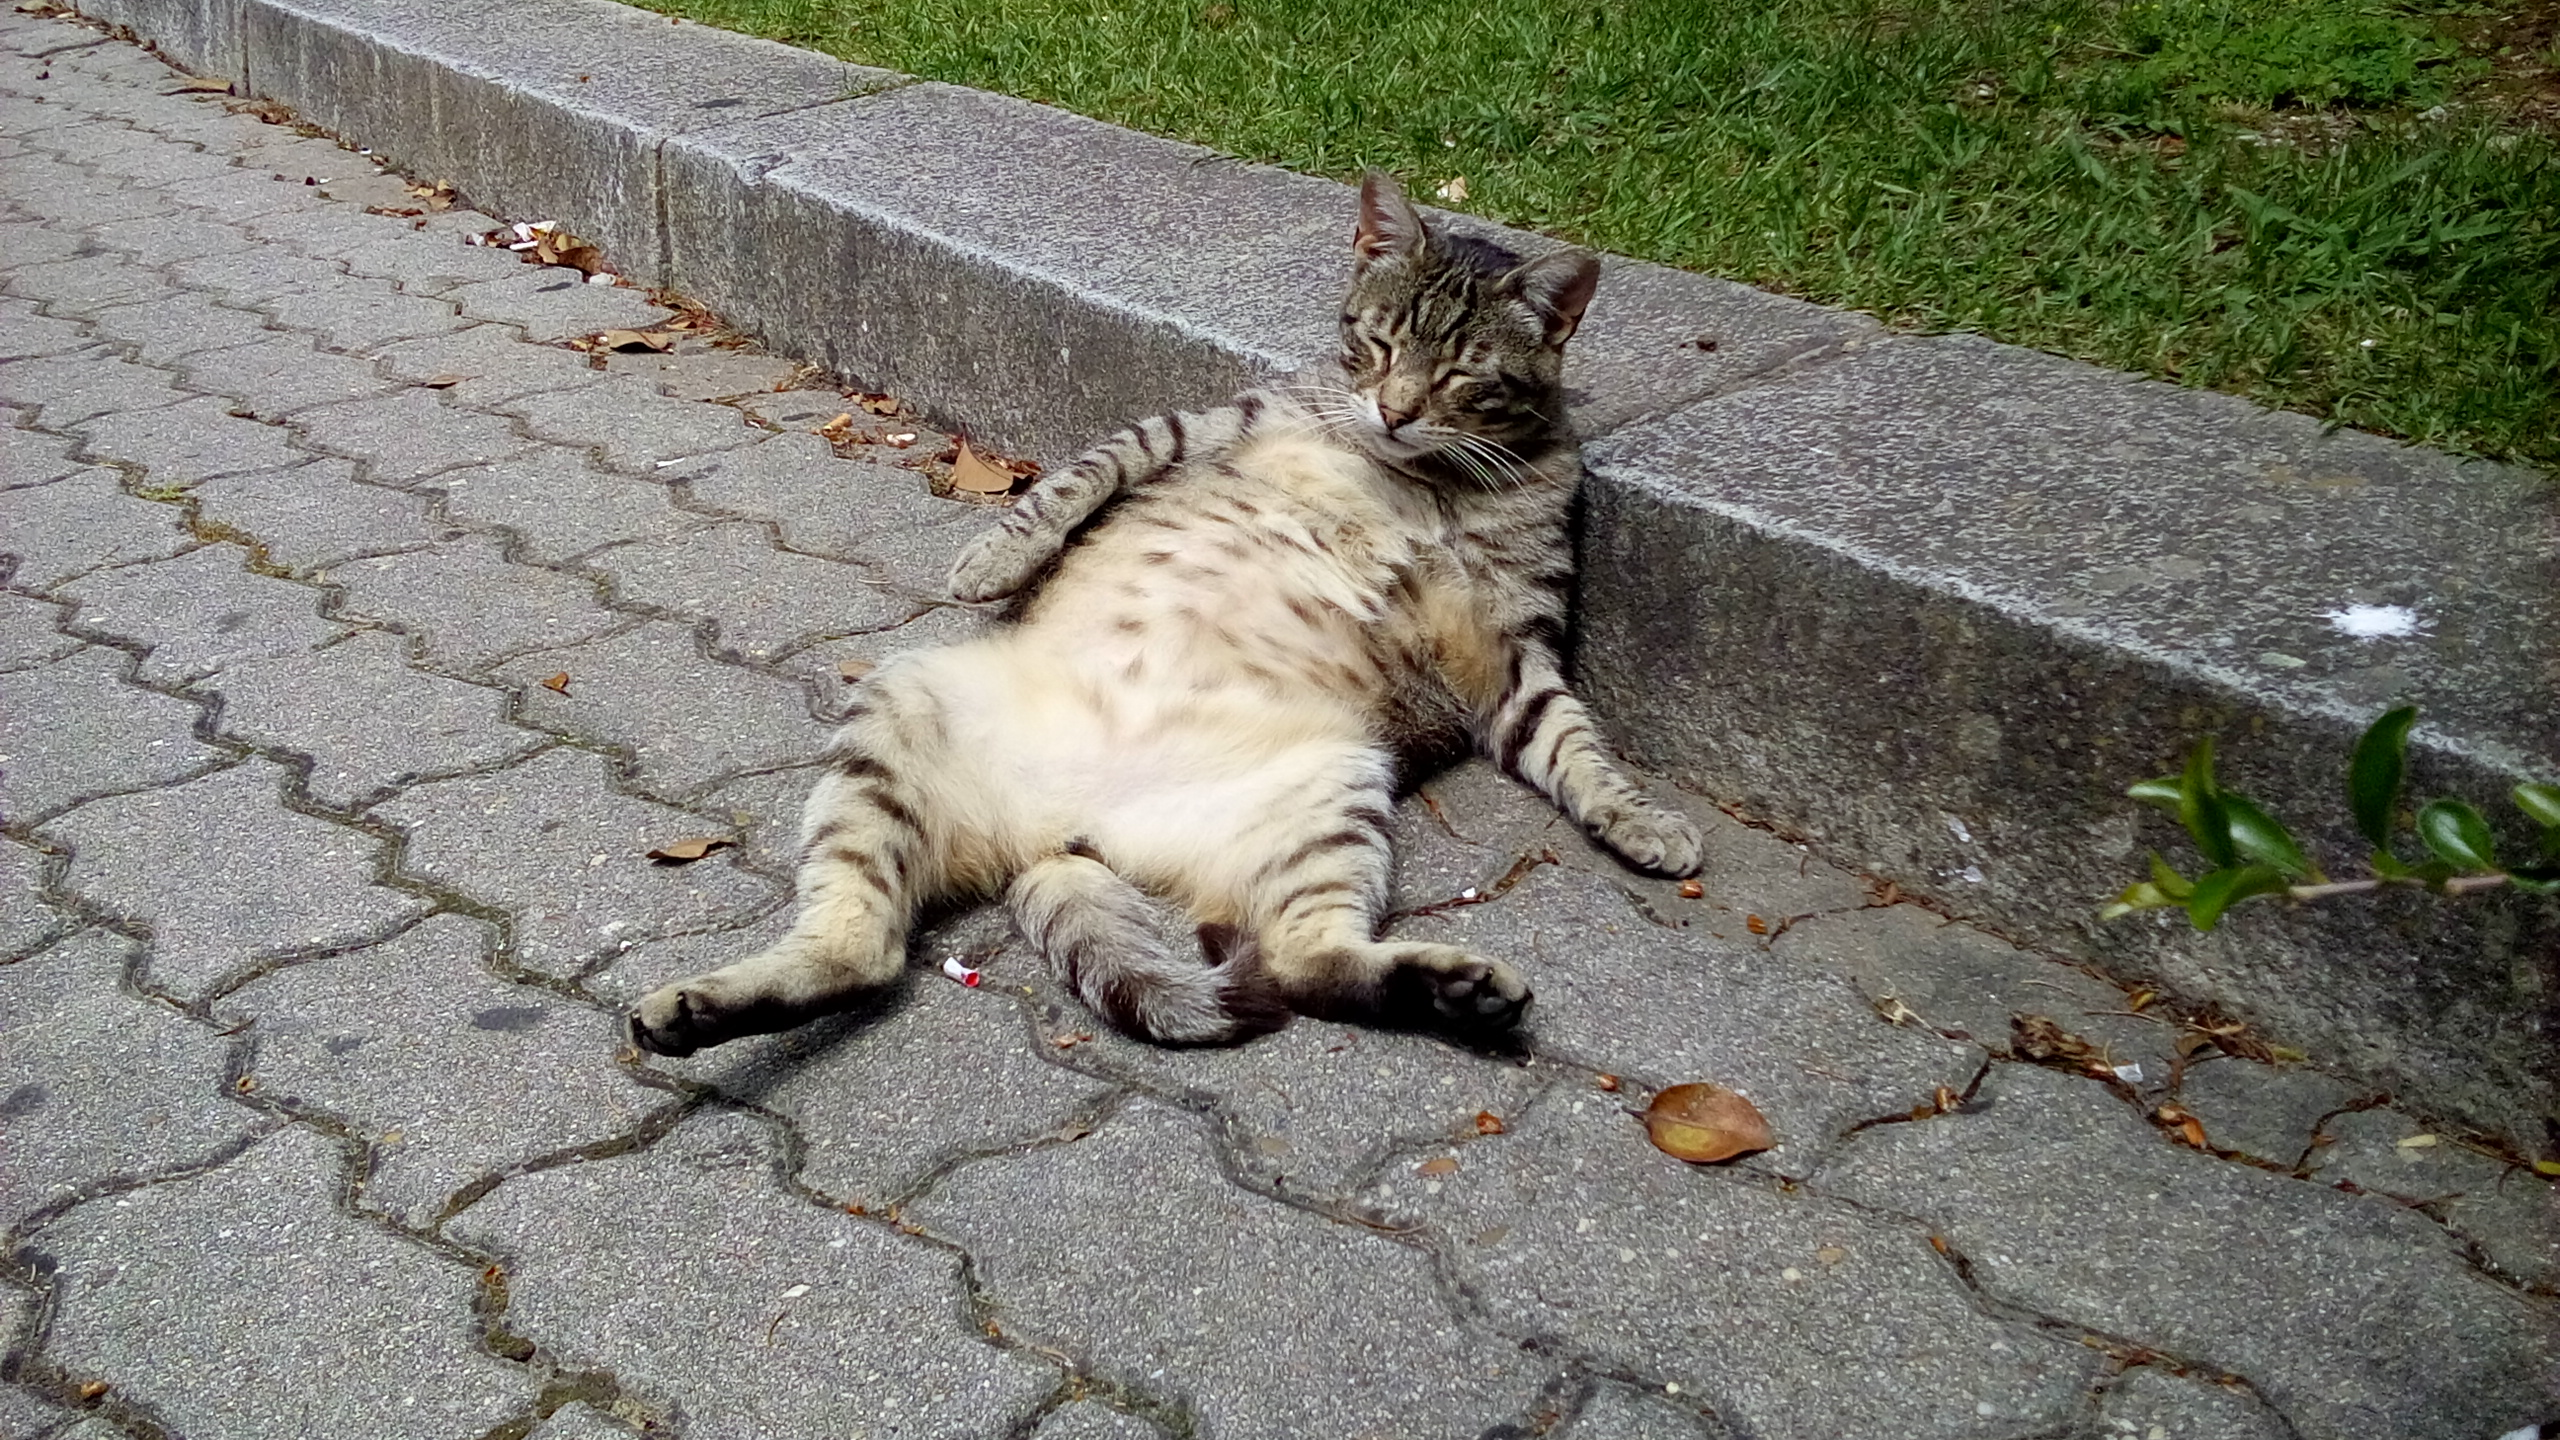
\includegraphics[width=8cm]{Figures/ChapterTemplate/20160517_123609.jpg}
  \captionof{figure}{\label{fig:FCUPfatcatSide4}FCUP's fat cat.} 
\end{wrapfigure} 
\lipsum[2-3]

\section{Math}


The following equation uses a custom mathematical operator defined in line 166 of the stock main.tex:
\begin{equation}
\begin{aligned}
			\meshgrid_{\mathbf{x}_{1},\mathbf{x}_{2}}\mathbf{x}_{1}&=\begin{bmatrix}a_{1} & b_{1} & c_{1}\\
a_{1} & b_{1} & c_{1}
\end{bmatrix}\\
			\meshgrid_{\mathbf{x}_{1},\mathbf{x}_{2}}\mathbf{x}_{2}&=\begin{bmatrix}a_{2} & a_{2} & a_{2}\\
b_{2} & b_{2} & b_{2}
\end{bmatrix}
\end{aligned}
\end{equation}

The following equation uses the custom ceil and floor operator defined in line 168 of the stock main.tex:

\begin{equation}
x = \floor*{\frac{y}{2}} + \ceil*{\frac{w}{2}}
\end{equation}


And this is an equation with multiple lines:
\begin{equation}
\begin{aligned}
&I_{0}=I^{\prime}+I^{\prime\prime}\cos(\varPsi)   \\
&I_{\pi/2}=-I^{\prime\prime}\sin(\varPsi)                \\
&I_{\pi}=I^{\prime}-I^{\prime\prime}\cos(\varPsi)   \\
&I_{3\pi/2}=I^{\prime\prime}\sin(\varPsi)
\end{aligned}
\end{equation}

